%% ----------------------------------------------------------------
%% AppendixAuthoringToolWireframes.tex
%% ---------------------------------------------------------------- 
\chapter{Authoring Tool Wireframes} \label{Chapter:Authoring Tool Wireframes}

\begin{preamble}
	An appendix showing the initial authoring tool wireframes.
\end{preamble}

\section{Introduction}

Wireframes were created to allow for feedback from users and the customer regarding potential designs for the Authoring tool.

\section{First Option} 

The first option we considered was using an accordian view shown in \autoref{Figure:wireframes/authoringtool/accordian}. Here the options for each part of the question sets are shown in accordians that appear as you edit the specific parts of the quiz.

\begin{figure}
	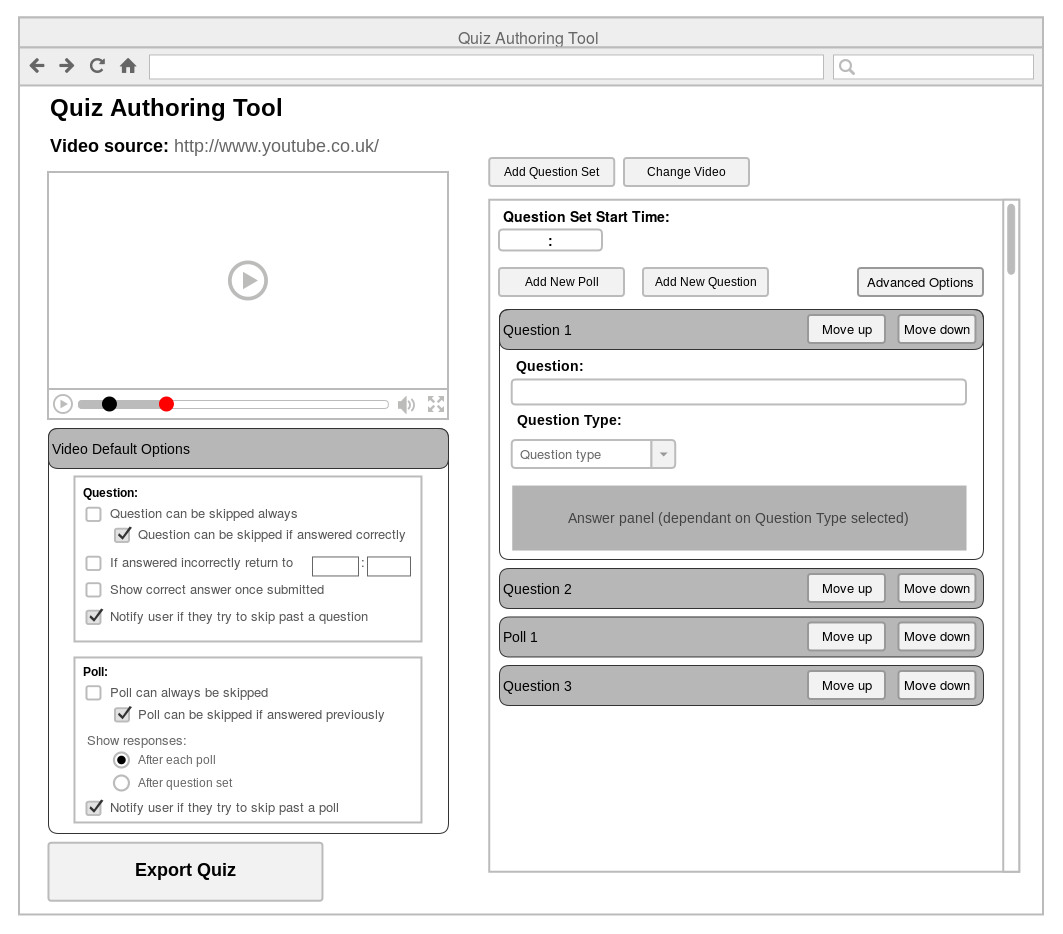
\includegraphics[width=\textwidth]{wireframes/gdpAuthoringAccordianVideoDefaultOptions.png}
	\caption{Wireframe showing the accordion type design of showing/hiding options}
	\label{Figure:wireframes/authoringtool/accordian}
\end{figure}

\section{Second Option}

We considered a second option where you would press an edit button and the options would pop up. Here you originally see the main screen shown in \autoref{Figure:wireframes/authoringtool/main} and then once you select an options button such as the ``advanced option'' button, you would see the popup shown in \autoref{Figure:wireframes/authoringtool/mainPopup}.

\begin{landscape}

\begin{figure}
	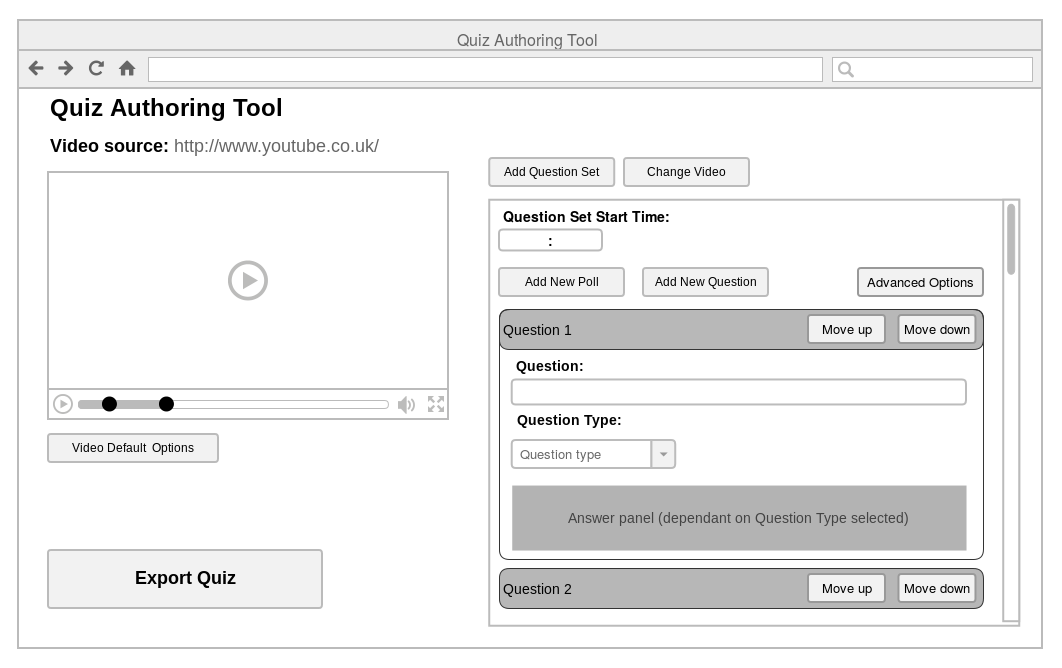
\includegraphics[width=22cm]{wireframes/gdpAuthoringMain.png}
	\caption{Wireframe showing the pop type design of showing/hiding options before opening a popup.}
	\label{Figure:wireframes/authoringtool/main}
\end{figure}

\begin{figure}
	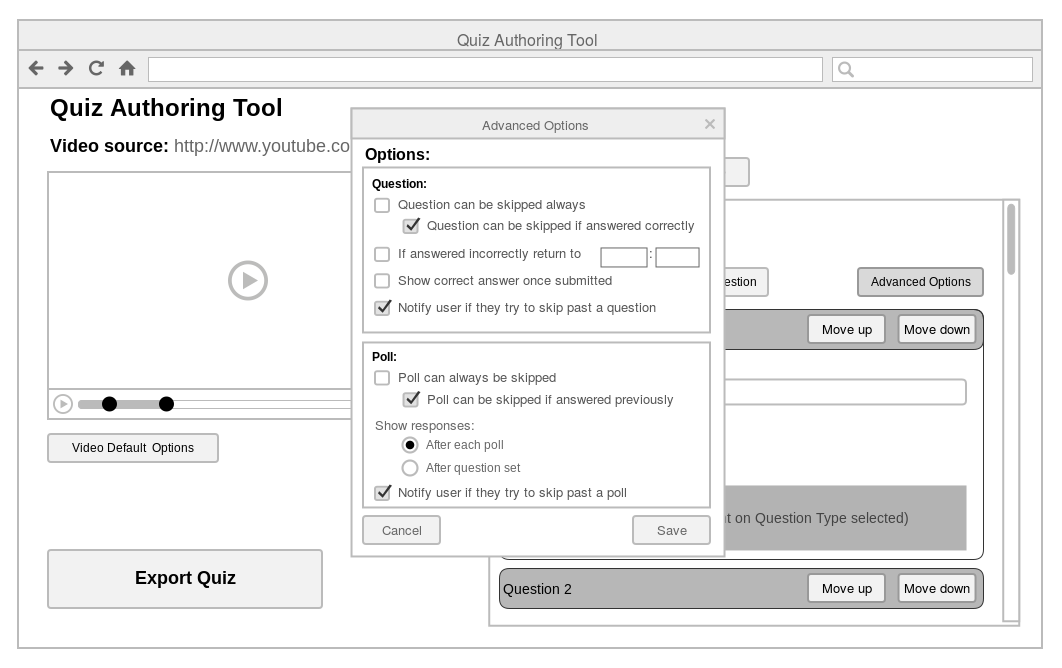
\includegraphics[width=22cm]{wireframes/gdpAuthoringAdvancedOptions.png}
	\caption{Wireframe showing the accordion type design of showing/hiding options after opening a popup.}
	\label{Figure:wireframes/authoringtool/mainPopup}
\end{figure}
\end{landscape}


\section{Question Creation wireframes}

These first wireframes (\autoref{Figure:wireframes/authoringtool/singlePoll}, \autoref{Figure:wireframes/authoringtool/singleQuiz}, \autoref{Figure:wireframes/authoringtool/multiPoll}, \autoref{Figure:wireframes/authoringtool/multiQuiz}, \autoref{Figure:wireframes/authoringtool/rangeStarPoll}, \autoref{Figure:wireframes/authoringtool/rangeStarQuiz}) show how the questions were originally planned to look. This demonstrates the differences between the poll and quiz type options, where the quiz type questions allow the choice of a "correct" answer. These were used to generate the first iteration of HTML mockups, once we had the mockups we used the HTML and iterated over them. This was because it was easier to have more realistic models to present to users and the client.

\begin{figure}
	\centering
	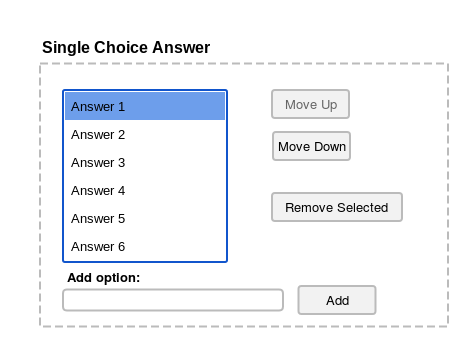
\includegraphics[width=12cm]{wireframes/gdpauthoringsingleanswerpoll.png}
	\caption{A wireframe showing the possible interface when creating a single choice poll type question}
	\label{Figure:wireframes/authoringtool/singlePoll}
\end{figure}

\begin{figure}
	\centering
	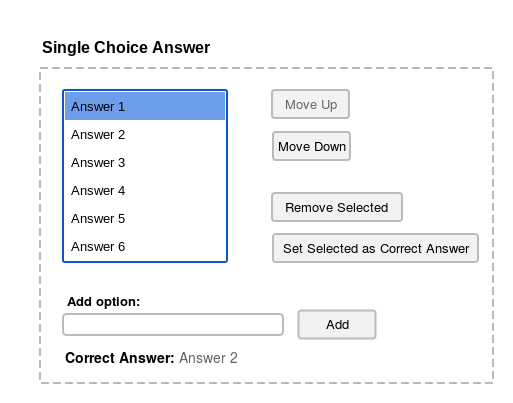
\includegraphics[width=12cm]{wireframes/gdpauthoringsingleanswerquestion.png}
	\caption{A wireframe showing the possible interface when creating a single choice quiz type question}
	\label{Figure:wireframes/authoringtool/singleQuiz}
\end{figure}

\begin{figure}
	\centering
	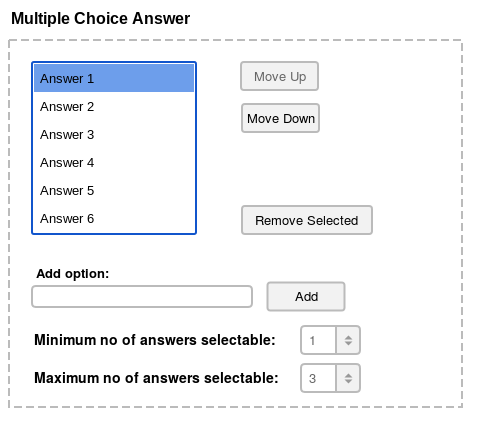
\includegraphics[width=10cm]{wireframes/gdpauthoringmultianswerpoll.png}
	\caption{A wireframe showing the possible interface when creating a multiple choice poll type question}
	\label{Figure:wireframes/authoringtool/multiPoll}
\end{figure}

\begin{figure}
	\centering
	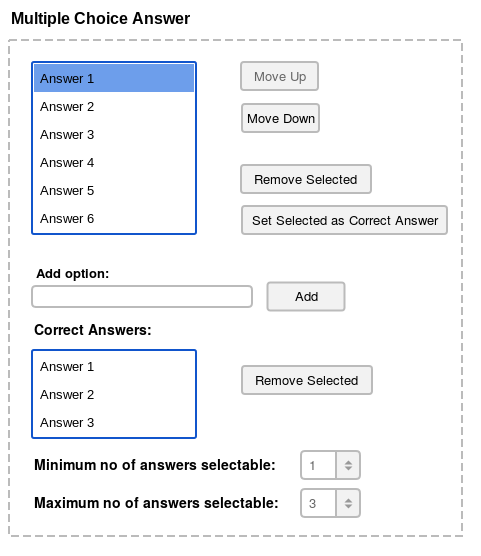
\includegraphics[width=10cm]{wireframes/gdpauthoringmultianswerquestion.png}
	\caption{A wireframe showing the possible interface when creating a multiple choice quiz type question}
	\label{Figure:wireframes/authoringtool/multiQuiz}
\end{figure}

\begin{figure}
	\centering
	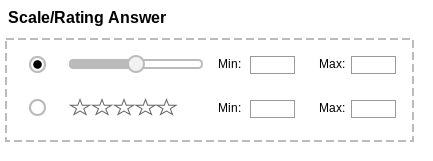
\includegraphics[width=10cm]{wireframes/gdpauthoringscalepoll.png}
	\caption{A wireframe showing the possible interface when creating a range or star poll type question}
	\label{Figure:wireframes/authoringtool/rangeStarPoll}
\end{figure}


\begin{figure}
	\centering
	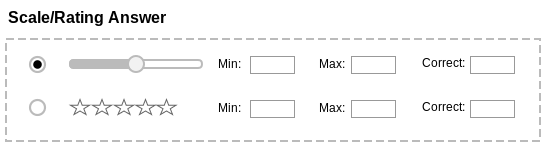
\includegraphics[width=12cm]{wireframes/gdpauthoringscalequestion.png}
	\caption{A wireframe showing the possible interface when creating a range or star quiz type question}
	\label{Figure:wireframes/authoringtool/rangeStarQuiz}
\end{figure}

\section{Accessibility Tooltips}

To aid accessibility we have planned to make tooltips appear on elements. This was illustrated in the example tooltip wireframe \autoref{Figure:wireframes/authoringtool/tooltip}.

\begin{landscape}
\begin{figure}
	\centering
	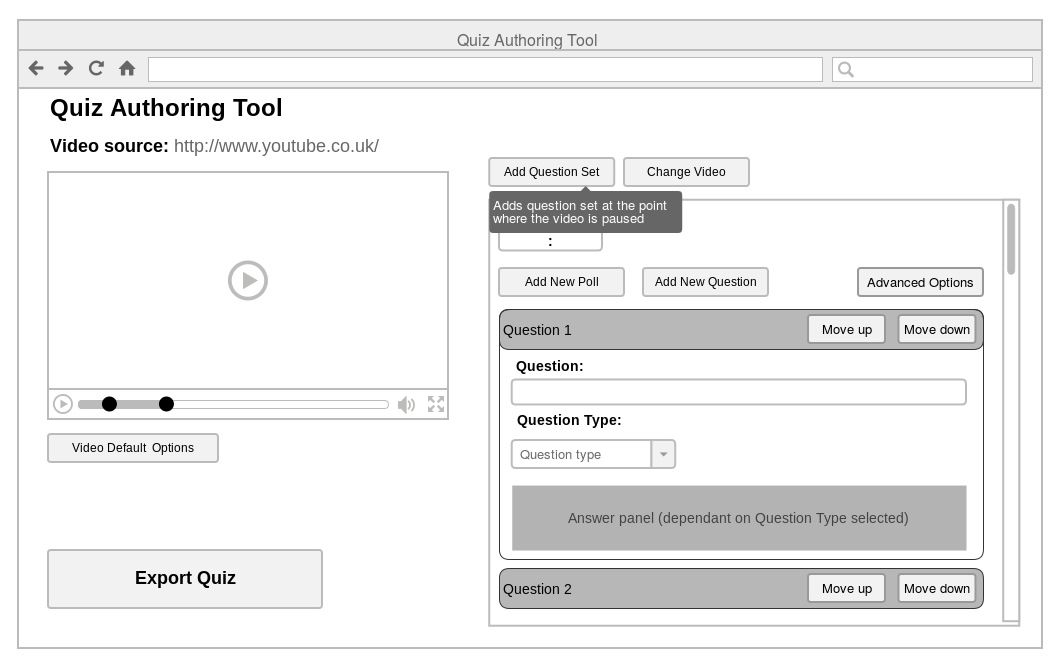
\includegraphics[width=22cm]{wireframes/gdpAuthoringToolTip.png}
	\caption{A wireframe showing an example of how tooltips could be implemented}
	\label{Figure:wireframes/authoringtool/tooltip}
\end{figure}
\end{landscape}
